\documentclass[24pt,pdf,hyperref={unicode}]{beamer}
\usepackage[utf8]{inputenc}
\usepackage{aiml}

\begin{document}


\section{Персептрон}

\begin{frame}\frametitle{Персептрон}
\begin{columns}
\column{0.4\textwidth}
\begin{tikzpicture}
\node[neu] (n) at (1,0) {$n$};
\foreach \x in {1,...,3}
	{
	\node (x-\x) at (-1,2-\x) {$x_\x$};
	\path (x-\x) edge[->] node[above,near start] {$w_\x$} (n);
	}
\node (y) at (2,0) {$y$};
\path (n) edge[->] (y);
\end{tikzpicture}
$$
y=f\left(\sum_{i=1}^{n}w_ix_i\right)
$$
\column{0.6\textwidth}

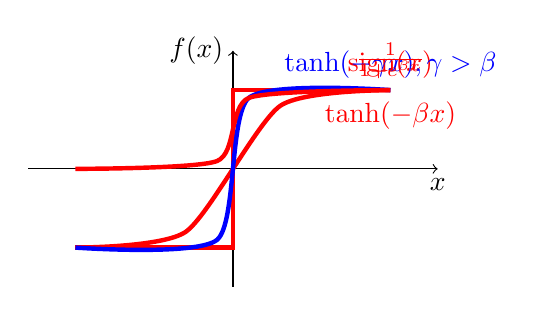
\begin{tikzpicture}[x=2cm,y=1cm]
\draw[->] (-1.3,0) -- (1.3,0) node[below] {$x$};
\draw[->] (0,-1.5) -- (0,1.5) node[left] {$f(x)$};

\uncover<+>{
\draw[ultra thick,red] plot coordinates {(-1,-1) (0,-1) (0,1) (1,1) } node[above] {${\rm sign}(x)$};
}

\uncover<2-3>{
\draw[ultra thick,red,smooth,tension=0.4] plot coordinates {(-1,-1) (-0.3,-0.8) (0.3,0.8) (1,1) } node[below] {${\rm tanh}(-\beta x)$};
}

\uncover<3>{
\draw[ultra thick,blue,smooth,tension=0.4] plot coordinates {(-1,-1) (-0.1,-0.9) (0.1,0.9) (1,1) } node[above] {${\rm tanh}(-\gamma x),\gamma>\beta$};
}

\uncover<4>{
\draw[ultra thick,red,smooth,tension=0.4] plot coordinates {(-1,0) (-0.1,0.1) (0.1,0.9) (1,1) } node[above] {$\frac{1}{1+e^{\beta x}}$};
}


\end{tikzpicture}

\end{columns}
\end{frame}


\begin{frame}\frametitle{Вес активации}
\begin{center}
\begin{tikzpicture}[scale=2]
\node[neu] (n) at (1,0) {$n$};
\foreach \x in {1,...,3}
	{
	\node (x-\x) at (-1,2-\x) {$x_\x$};
	\path (x-\x) edge[->] node[above,near start] {$w_\x$} (n);
	}
\node (y) at (2,0) {$y$};
\path (n) edge[->] (y);
\uncover<2>{
\node (x-0) at (-1,2) {$x_0\equiv 1$};
\path (x-0) edge[->] node[above,near start] {$w_0$} (n);
} 
\end{tikzpicture}
\end{center}
\end{frame}

\begin{frame}\frametitle{Реализация конъюнкции}
\begin{columns}
\column{0.5\textwidth}
$$
\begin{array}{c c | c}
x_1 & x_2 & x_1\wedge x_2 \\
\hline
0 & 0 & 0 \\
0 & 1 & 0 \\
1 & 0 & 0 \\
1 & 1 & 1 \\
\end{array}
$$
\column{0.5\textwidth}
$$
\left\{
\begin{array}{l l l l l l}
 w_0       & < & 0 \\
 w_0 + w_1 & < & 0 \\
 w_0 + w_2 & < & 0 \\
 w_0 + w_1 + w_2 & > & 0 \\
\end{array}
\right.
$$\\[1cm]
\uncover<2>{
$$
\begin{array}{l}
 w_0 = 3 \\
 w_1 = 2 \\
 w_2 = 2 \\
\end{array}
$$
}
\end{columns}
\end{frame}


\begin{frame}\frametitle{Реализация дизъюнкции}
\begin{columns}
\column{0.5\textwidth}
$$
\begin{array}{c c | c}
x_1 & x_2 & x_1\vee x_2 \\
\hline
0 & 0 & 0 \\
0 & 1 & 1 \\
1 & 0 & 1 \\
1 & 1 & 1 \\
\end{array}
$$
\column{0.5\textwidth}
$$
\left\{
\begin{array}{l l l l l l}
 w_0       & < & 0 \\
 w_0 + w_1 & > & 0 \\
 w_0 + w_2 & > & 0 \\
 w_0 + w_1 + w_2 & > & 0 \\
\end{array}
\right.
$$\\[1cm]
$$
\begin{array}{l}
 w_0 = 1 \\
 w_1 = 2 \\
 w_2 = 2 \\
\end{array}
$$
\end{columns}
\end{frame}

\begin{frame}\frametitle{Геометрическая интерпретация}
\uncover<+->{}
\begin{tikzpicture}[y=4cm, x=4cm]
\draw[->] (-0.1,0) -- (1.5,0) node[below]{$x_1$};
\draw[->] (0,-0.1) -- (0,1.5) node[left]{$x_2$};
\draw[fill=black] (0,0) circle(3pt);
\draw[fill=black] (0,1) circle(3pt);
\draw[fill=black] (1,0) circle(3pt);
\draw[fill=white] (1,1) circle(3pt);

\uncover<+->{
\draw (0.1,1.4) -- (1.4,0.1);
\draw[->] (0.75,0.75) -- (0.85,0.85) node[right] {$(w_1,w_2)$};
}
\end{tikzpicture}
\end{frame}

\begin{frame}\frametitle{Обучение персептрона}
Тут про советчиков, м.б. тоже в PP
\end{frame}

\end{document}